\documentclass[11pt]{article}

\usepackage[a4paper,margin=1in]{geometry}
\usepackage[T1]{fontenc}
\usepackage[utf8]{inputenc}
\usepackage{lmodern}
\usepackage{microtype}
\usepackage{amsmath,amssymb,amsthm,mathtools}
\usepackage{booktabs}
\usepackage{array}
\usepackage{graphicx}
\usepackage{float}
\usepackage{placeins}
\usepackage{enumitem}
\usepackage[numbers,sort&compress]{natbib}
\usepackage{xcolor}
\usepackage{xurl}
\usepackage[colorlinks=true,linkcolor=blue!55!black,citecolor=blue!55!black,urlcolor=blue!55!black]{hyperref}
\usepackage[nameinlink,noabbrev]{cleveref}

\setlength{\parindent}{1.4em}
\setlength{\parskip}{0.15em}
\setlist{itemsep=0.25em,topsep=0.35em}
\allowdisplaybreaks

\newtheorem{theorem}{Theorem}[section]
\newtheorem{proposition}[theorem]{Proposition}
\newtheorem{lemma}[theorem]{Lemma}
\newtheorem{corollary}[theorem]{Corollary}
\theoremstyle{definition}
\newtheorem{definition}[theorem]{Definition}
\theoremstyle{remark}
\newtheorem{remark}[theorem]{Remark}

\newcommand{\C}{\mathbb C}
\newcommand{\Id}{\mathrm I}
\newcommand{\norm}[1]{\left\lVert#1\right\rVert}
\newcommand{\wind}{\operatorname{wind}}
\newcommand{\spec}{\operatorname{spec}}
\newcommand{\Rapp}{\mathcal R}
\newcommand{\Gmat}{\mathcal G}
\newcommand{\Lmat}{\mathcal L}
\newcommand{\Maug}{\mathcal M_{\rm st}}

\hypersetup{
  pdftitle={A Certified Complement-Resolvent Atlas and a Relative Contour Count},
  pdfauthor={Liang Wang},
  pdfsubject={Full-boundary outward-rounded resolvent closure and an exact stored-block relative count},
  pdfkeywords={resolvent atlas, Grushin problem, Feshbach map, matrix Rouche theorem, verified numerics, nonnormal matrix}
}

\title{\textbf{A Certified Complement-Resolvent Atlas and a\\
Relative Contour Count}\\[0.35em]
\large Full-Boundary Rouch\'e Closure for a 2048-Dimensional\\
Stored Quadratic Band-Merging Model}
\author{Liang Wang\\
\small School of Artificial Intelligence and Automation,\\[-0.2em]
\small Huazhong University of Science and Technology, Wuhan 430074, P.R. China\\
\small \texttt{wangliang.f@gmail.com}}
\date{July 2026}

\begin{document}
\maketitle

\begin{abstract}
An end-to-end certificate ledger for a finite packet--complement spectral
model left two independent gates: a validated complement-resolvent bound on
the complete contour, and an interior count of complement poles.  This paper
closes the first gate at the stored scale $\sigma=10^{-2}$.

Let $M$ be the stored sparse one-step matrix,
$U=M-R_{\rm p}\Lambda L_{\rm p}^{\mathsf T}$,
$Q=\Id-VW$, and $B=QU^2Q$.  No exact idempotence of the stored $Q$ is
assumed.  For $A(z)=z\Id-B$, we use the unlifted two-step linearization
\[
 \mathcal L_t(z)=
 \begin{pmatrix}z\Id&-tQU\\-t^{-1}UQ&\Id\end{pmatrix}.
\]
Its leading inverse block is $A(z)^{-1}$.  The off-diagonal factors are a
sparse $M$ block plus $2p+2m=12$ peripheral and packet channels.  A bordered
Grushin realization therefore has dimension $4108$ when the physical
dimension is $2048$.

At each of 109 contour centers, sparse LU is used only to generate a
binary64 trial right inverse $\mathcal R_j$.  The exact stored-factor graph
then independently encloses
$\Id-A(z_j)\mathcal R_j$ componentwise.  All 109 residual Frobenius bounds
are below $5.747\times10^{-9}$, and the resulting rigorous inverse bounds
range from $50.486$ to $553.228$.  These local certificates are transported
with 256-bit Arb arithmetic to an exact rational cover.  Of 936 inherited
RH-28 parent arcs, 933 close without further subdivision; the remaining
three close after dyadic refinement.  The final cover has 949 leaves, no
gap, and no unresolved leaf.  Its largest rigorous Neumann product is
$0.999870853<1$, while the largest transported-bound-to-RH-28-budget ratio is
$2.107\times10^{-11}$.

Consequently the RH-28 matrix Rouch\'e inequality holds on the entire stored
circle.  Combining this with the independently certified RH-32 projected
winding gives $\wind_\Gamma\det F=1$ for the exact stored Feshbach function.
Moreover, for the exact augmented block realization
\[
 \mathcal M_{\rm st}=\begin{pmatrix}D&E\\C&B\end{pmatrix},
\]
the Schur determinant identity yields the rigorous relative count
\[
 N_\Gamma(\mathcal M_{\rm st})-N_\Gamma(B)=1.
\]
This is a full-boundary and relative-count theorem, not an ordinary one-zero
theorem: the interior complement count remains open.  No continuum limit,
Hilbert--P\'olya construction, zeta-zero identification, Riemann-hypothesis
implication, or one-eigenvalue claim for the original physical
discretization is made.
\end{abstract}

\noindent\textbf{Keywords:} complement resolvent; certified atlas; Grushin
problem; Feshbach map; matrix Rouch\'e theorem; verified numerical linear
algebra; nonnormal spectrum.

\medskip
\noindent\textbf{MSC 2020:} 15A18; 47A10; 47A11; 47A55; 65F05; 65F35;
65F50; 65G20; 65P30.

\section{Introduction}
\label{sec:introduction}

The contour program considered here studies a finite noisy transfer matrix
near a quadratic band-merging parameter.  A small packet block is retained,
the ambient complement is eliminated by a Feshbach map, and a rational
Arnoldi realization supplies a tractable projected determinant.  Successive
papers made the comparison more explicit: primal--dual identities isolated
the complement inverse, outward arithmetic enclosed the stored residuals,
and exact rational arcs replaced sampled contour nodes
\citep{WangContourFeshbach2026,WangOutwardCode2026,WangArcwise2026}.

The remaining inverse problem is genuinely nonnormal.  A one-channel lift
and sparse two-step Grushin linearization certified selected centers, while a
threshold-inertia route provided independent local certificates
\citep{WangDeflated2026,WangSparseGrushin2026,WangThresholdInertia2026}.
The end-to-end ledger then made the limitation precise: one selected center
reached only one RH-28 arc, so it could not be promoted to a complete
contour theorem \citep{WangLedger2026}.

The natural next object is not one especially sharp center but a finite
\emph{resolvent atlas}.  Each chart consists of a validated inverse bound at
one center together with the neighborhood reached by the resolvent identity.
Compactness suggests that finitely many charts should cover a pole-free
boundary; the difficulty is to certify every chart without assembling the
dense square $QU^2Q$ or trusting a computed smallest singular value.

This paper implements that route at $\sigma=10^{-2}$.  Its contributions
are:

\begin{enumerate}
 \item an unlifted sparse two-step Grushin realization with exact physical
       inverse block $A(z)^{-1}$ and only $2p+2m$ low-rank channels;
 \item 109 deterministic all-column Frobenius--Neumann certificates whose
       residuals are reevaluated against the exact stored-factor target;
 \item a rational adaptive atlas that may place new centers inside RH-28
       parent arcs rather than only at archived parent midpoints;
 \item a 256-bit Arb transport audit proving a complete 949-leaf cover of
       the stored circle;
 \item full-boundary activation of the RH-28 matrix Rouch\'e inequality;
 \item an exact winding-one theorem for the stored Feshbach function and an
       exact augmented-block-minus-complement eigenvalue count of one; and
 \item an explicit separation of that relative count from the still-open
       interior complement count.
\end{enumerate}

The evidence hierarchy is maintained throughout.

\begin{itemize}
 \item Schur complements, low-rank channel identities, the resolvent
       transport, boundary homotopy, and relative count are exact algebra.
 \item Center residuals and the final atlas are rigorous computer-assisted
       results for exact serialized binary64 inputs under the stated IEEE
       arithmetic assumptions.
 \item Sparse LU factors and timings are computational devices and
       diagnostics.  No floating singular value is used as an upper bound.
\end{itemize}

\section{Exact stored Feshbach function and relative count}
\label{sec:stored-model}

Fix the stored scale $\sigma=10^{-2}$ and let $n=2048$.  The serialized
factors are interpreted componentwise as exact dyadic real or complex
numbers.  Let $M\in\C^{n\times n}$ be the sparse one-step matrix, let
$R_{\rm p},L_{\rm p}\in\C^{n\times p}$ with $p=2$ be the stored peripheral
factors, and let $\Lambda\in\C^{p\times p}$ contain their stored values.  Put
\begin{equation}
 U=M-R_{\rm p}\Lambda L_{\rm p}^{\mathsf T}.
 \label{eq:stored-u}
\end{equation}
The packet synthesis and analysis matrices are
$V\in\C^{n\times m}$ and $W\in\C^{m\times n}$ with $m=4$, and
\begin{equation}
 Q=\Id-VW.
 \label{eq:stored-q}
\end{equation}
As in the outward-rounded stored-factor model, no exact idempotence of $Q$
is assumed.  Define
\begin{equation}
 B=QU^2Q,\qquad C=QU^2V,\qquad D=WU^2V,\qquad E=WU^2Q.
 \label{eq:stored-blocks}
\end{equation}
For
\begin{equation}
 A(z)=z\Id_n-B,
 \label{eq:complement-shift}
\end{equation}
the exact stored Feshbach function is
\begin{equation}
 F(z)=z\Id_m-D-EA(z)^{-1}C
 \label{eq:stored-feshbach}
\end{equation}
wherever $A(z)$ is invertible.

Even without assuming that $Q$ is a projector, this rational function has
an exact block realization.  Set
\begin{equation}
 \Maug=
 \begin{pmatrix}
  D&E\\ C&B
 \end{pmatrix}
 \in\C^{(m+n)\times(m+n)}.
 \label{eq:stored-augmented-block}
\end{equation}

\begin{proposition}[Exact stored-block Schur identity]
\label{prop:stored-schur}
For $z\notin\spec B$,
\begin{equation}
 \det(z\Id_{m+n}-\Maug)=\det A(z)\det F(z).
 \label{eq:stored-schur-determinant}
\end{equation}
If a positively oriented simple contour $\Gamma$ meets neither
$\spec B$ nor $\spec\Maug$, then
\begin{equation}
 \wind_\Gamma\det F=N_\Gamma(\Maug)-N_\Gamma(B).
 \label{eq:stored-relative-count}
\end{equation}
\end{proposition}

\begin{proof}
The matrix $z\Id_{m+n}-\Maug$ has block form
\[
 \begin{pmatrix}
  z\Id_m-D&-E\\ -C&z\Id_n-B
 \end{pmatrix}.
\]
Taking the Schur complement of $A(z)=z\Id_n-B$ gives
\cref{eq:stored-schur-determinant}.  Both determinants in the quotient are
polynomials, so the scalar argument principle gives
\cref{eq:stored-relative-count}
\citep{Ahlfors1979,HornJohnson2013}.
\end{proof}

\begin{remark}[What the augmented block is]
\label{rem:augmented-scope}
The matrix $\Maug$ is the exact finite block realization of the stored
function \cref{eq:stored-feshbach}.  If $WV=\Id_m$ exactly, it is the usual
oblique-coordinate representation of the physical two-step operator.  The
serialized stored model does not assume that exact identity, so the present
paper does not silently identify $\Maug$ with the original physical
discretization.
\end{remark}

The projected rational Feshbach function $F_J$ and the circle $\Gamma$ are
inherited from RH-28.  RH-32 reconstructed the exact RH-28 base realization,
enclosed all augmented and pole eigenvalues with 256-bit Arb arithmetic, and
proved at the present scale that
\begin{equation}
 \wind_\Gamma\det F_J=1,\qquad
 \det F_J(z)\ne0\quad(z\in\Gamma).
 \label{eq:projected-winding-one}
\end{equation}
The circle has stored center and radius
\begin{equation}
 c=-0.3233504401504541-0.5508412474453575i,\qquad
 R=0.2624987592858511.
 \label{eq:stored-circle}
\end{equation}
The task below is to transfer \cref{eq:projected-winding-one} to $F$ on the
entire boundary.

\section{Unlifted sparse two-step Grushin realization}
\label{sec:grushin}

For $t>0$ and a spectral parameter $z$, define
\begin{equation}
 \Lmat_t(z)=
 \begin{pmatrix}
  z\Id_n&-tQU\\
  -t^{-1}UQ&\Id_n
 \end{pmatrix}.
 \label{eq:two-step-linearization}
\end{equation}

\begin{lemma}[Physical inverse block]
\label{lem:physical-inverse}
The Schur complement of the lower-right identity in
\cref{eq:two-step-linearization} is $A(z)$.  Consequently
$\Lmat_t(z)$ is invertible if and only if $A(z)$ is invertible, and
\begin{equation}
 [\Lmat_t(z)^{-1}]_{11}=A(z)^{-1}.
 \label{eq:leading-inverse-block}
\end{equation}
\end{lemma}

\begin{proof}
The Schur complement is
\[
 z\Id_n-(-tQU)(-t^{-1}UQ)=z\Id_n-QU^2Q=A(z).
\]
The block inverse formula gives \cref{eq:leading-inverse-block}.
\end{proof}

The dense-looking factors $QU$ and $UQ$ are low-rank corrections of the
sparse matrix $M$.  Write $C_{\rm p}=R_{\rm p}\Lambda$.  Exact algebra gives
\begin{align}
 M-QU&=C_{\rm p}L_{\rm p}^{\mathsf T}+V(WU),
 \label{eq:top-correction}\\
 M-UQ&=C_{\rm p}L_{\rm p}^{\mathsf T}+(UV)W.
 \label{eq:bottom-correction}
\end{align}
Define the sparse base
\begin{equation}
 \Lmat_{0,t}(z)=
 \begin{pmatrix}
  z\Id_n&-tM\\
  -t^{-1}M&\Id_n
 \end{pmatrix}.
 \label{eq:sparse-base}
\end{equation}
Equations \cref{eq:top-correction,eq:bottom-correction} express
$\Lmat_t(z)-\Lmat_{0,t}(z)$ as $XY$ with
\begin{equation}
 X\in\C^{2n\times r},\qquad Y\in\C^{r\times2n},\qquad r=2p+2m=12.
 \label{eq:channel-rank}
\end{equation}
The explicit channels are listed in \cref{app:channels}.

\begin{theorem}[Sparse unlifted Grushin inverse]
\label{thm:sparse-grushin}
Let
\begin{equation}
 \Gmat_t(z)=
 \begin{pmatrix}
  \Lmat_{0,t}(z)&X\\
  Y&-\Id_r
 \end{pmatrix}.
 \label{eq:bordered-grushin}
\end{equation}
Let $J_n:\C^n\to\C^{2n+r}$ inject into the first $n$ coordinates.  Then
$\Gmat_t(z)$ is invertible if and only if $A(z)$ is invertible, and
\begin{equation}
 J_n^*\Gmat_t(z)^{-1}J_n=A(z)^{-1}.
 \label{eq:grushin-physical-block}
\end{equation}
The bordered dimension is $2n+2p+2m=4108$.
\end{theorem}

\begin{proof}
The Schur complement of $-\Id_r$ is
$\Lmat_{0,t}(z)+XY=\Lmat_t(z)$.  Hence the leading $2n$ inverse block of
$\Gmat_t(z)^{-1}$ is $\Lmat_t(z)^{-1}$.  Apply
\cref{lem:physical-inverse} to its first $n$ coordinates.
\end{proof}

Each channel may be balanced by multiplying its column and dividing its row
by the same nonzero scalar.  This preserves $XY$ and the physical inverse
block.  The implementation chooses the square root of the row-to-column
Euclidean norm ratio.  The choice affects sparse factorization quality, not
the target of the final certificate \citep{Davis2006,WangSparseGrushin2026}.

\section{Direct exact-target center certificates}
\label{sec:center-certificates}

At a center $z_j$, a binary64 sparse LU factorization of
$\Gmat_1(z_j)$ solves
\begin{equation}
 \widehat{\Gmat}_1(z_j)x_k=J_ne_k,\qquad k=1,\ldots,n.
 \label{eq:trial-solves}
\end{equation}
Retaining the first $n$ coordinates produces a stored trial matrix
$\Rapp_j\in\C^{n\times n}$.  Neither the rounded assembly nor the LU factors
are asserted to be exact.

\begin{theorem}[Frobenius--Neumann right-inverse certificate]
\label{thm:frobenius-neumann}
Let $T,R\in\C^{n\times n}$.  If rigorous bounds $\rho,\varepsilon$ satisfy
\begin{equation}
 \norm{R}_F\leq\rho,\qquad
 \norm{\Id-TR}_F\leq\varepsilon<1,
 \label{eq:fn-inputs}
\end{equation}
then $T$ is invertible and
\begin{equation}
 \norm{T^{-1}}_2\leq\frac{\rho}{1-\varepsilon}.
 \label{eq:fn-bound}
\end{equation}
\end{theorem}

\begin{proof}
Let $\Delta=\Id-TR$.  Since
$\norm{\Delta}_2\leq\norm{\Delta}_F<1$, the Neumann lemma makes
$\Id-\Delta$ invertible and $T[R(\Id-\Delta)^{-1}]=\Id$.  A square matrix
with a right inverse is invertible.  Therefore
\[
 \norm{T^{-1}}_2
 \leq\norm{R}_2\norm{(\Id-\Delta)^{-1}}_2
 \leq\frac{\norm{R}_F}{1-\norm{\Delta}_F}.
\]
Apply \cref{eq:fn-inputs}.
\end{proof}

For the present target, the stored-factor graph reevaluates
\begin{equation}
 X\longmapsto z_jX-Q\bigl(U(U(QX))\bigr)
 \label{eq:exact-target-action}
\end{equation}
componentwise with one outward complex-disc radius per entry.  Sparse and
dense dot products use conservative Higham $\gamma_k$ factors, and every
positive bound operation is rounded outward
\citep{Higham2002,Rump2010}.  Thus the residual
\begin{equation}
 \Delta_j=\Id-A(z_j)\Rapp_j
 \label{eq:center-residual}
\end{equation}
is enclosed against the exact stored target, not against the rounded Schur
complement of the sparse LU matrix.

The 2048 physical columns are processed in chunks of 256.  Chunk Frobenius
bounds are combined by an outward square root of the sum of squares.  The
center bound is
\begin{equation}
 M_j=\frac{\rho_j}{1-\varepsilon_j},\qquad
 \rho_j\geq\norm{\Rapp_j}_F,\quad
 \varepsilon_j\geq\norm{\Delta_j}_F.
 \label{eq:center-bound}
\end{equation}

\begin{table}[H]
\centering
\caption{Stored sparse realization and all-center certificate ranges.  The
time entries are per center; the runs were performed in parallel batches.}
\label{tab:center-certificates}
\begin{tabular}{lr}
\toprule
quantity & certified or archived value\\
\midrule
physical dimension $n$ & 2048\\
packet rank $m$; peripheral rank $p$ & $4;\ 2$\\
border rank $r$; bordered dimension & $12;\ 4108$\\
bordered matrix nonzeros & 1,290,892\\
LU nonzeros, minimum--maximum & 3,672,780--3,672,782\\
number of center certificates & 109\\
$\rho_j$, minimum--maximum & 50.485781--553.227390\\
$\varepsilon_j$, minimum--maximum
 & $1.1195\times10^{-10}$--$5.7464\times10^{-9}$\\
$M_j$, minimum--maximum & 50.485781--553.227394\\
factor time per center & 2.26--2.36 s\\
exact-target certificate time per center & 27.15--31.35 s\\
\bottomrule
\end{tabular}
\end{table}

\begin{theorem}[109 direct center inverses]
\label{thm:center-inverses}
Assume the archived binary64 factors are exact inputs and IEEE
round-to-nearest arithmetic has no overflow or harmful underflow.  Every one
of the 109 archived center certificates is admissible.  In particular,
\begin{equation}
 50.485780584110735\leq M_j\leq553.2273931275126,
 \qquad j=1,\ldots,109,
 \label{eq:center-range}
\end{equation}
and each $A(z_j)$ is invertible.
\end{theorem}

\begin{proof}
For every center, the archived all-column calculation gives
$\varepsilon_j<5.747\times10^{-9}<1$.  Apply
\cref{thm:frobenius-neumann} to $T=A(z_j)$ and $R=\Rapp_j$.  The displayed
extrema are the outward bounds in the committed center manifest.
\end{proof}

\section{Adaptive rational resolvent atlas}
\label{sec:atlas}

The RH-28 boundary consists of 936 accepted parent arcs with exact rational
turn endpoints.  Parent $a$ lies on
\begin{equation}
 \gamma(\theta)=c+Re^{i\theta}
 \label{eq:circle-parameterization}
\end{equation}
and is enclosed by a stored disc
$\overline{\mathbb D}(\zeta_a,r_a)$.  It carries a downward conditional
budget $L_a^-$ such that
\begin{equation}
 \sup_{z\in a}\norm{A(z)^{-1}}_2<L_a^-
 \label{eq:rh28-resolvent-gate}
\end{equation}
activates the RH-28 matrix Rouch\'e inequality on that parent
\citep{WangArcwise2026}.

\begin{lemma}[One-chart disc transport]
\label{lem:chart-transport}
Suppose $\norm{A(z_j)^{-1}}_2\leq M_j$.  Let a target disc have center
$\zeta$ and radius $r$, and put
\begin{equation}
 d=|\zeta-z_j|+r.
 \label{eq:chart-distance}
\end{equation}
If $dM_j<1$, then every $z$ in the target disc satisfies
\begin{equation}
 \norm{A(z)^{-1}}_2\leq\frac{M_j}{1-dM_j}.
 \label{eq:chart-transport}
\end{equation}
\end{lemma}

\begin{proof}
Since $A(z)=A(z_j)+(z-z_j)\Id$, factor
\[
 A(z)=A(z_j)\bigl[\Id+(z-z_j)A(z_j)^{-1}\bigr].
\]
The Neumann lemma applies for $|z-z_j|M_j<1$, and every point of the target
disc has $|z-z_j|\leq d$.
\end{proof}

All quantities in \cref{eq:chart-distance,eq:chart-transport} are evaluated
with 256-bit Arb arithmetic.  Each binary64 real and imaginary component,
disc radius, center bound, and parent budget is embedded as its exact dyadic
value.  A target closes only when the upper Arb product is strictly below
one and the upper transported bound is strictly below the exact dyadic lower
budget.  Thus the final atlas does not rely on a plotted distance or a
single-successor approximation to a Euclidean norm \citep{Johansson2017}.

\subsection{Adaptive construction}

The construction begins with 64 approximately angle-uniform RH-28 parent
midpoints.  Additional parent midpoints are inserted at uncovered runs,
giving 88 parent-center certificates.  At that point a parent-only strategy
becomes inefficient: a large parent can fail as one disc even when smaller
subarcs are locally coverable.

The adaptive stage performs the following exact rational loop.

\begin{enumerate}
 \item Bisect every unresolved parent leaf up to a prescribed extra depth.
 \item Merge adjacent unresolved leaves by exact rational endpoint equality,
       including the $0/1$ turn seam.
 \item Place one new center at the rational-turn midpoint of each connected
       unresolved component.
 \item Certify every new center by \cref{thm:frobenius-neumann} and repeat.
\end{enumerate}

The first gap round contributes 13 centers and the second contributes 8.
Hence the final atlas consists of 88 parent midpoints and 21 adaptive
gap-midpoints.  Every one of the 109 centers is used by at least one final
leaf.

\subsection{Complete cover}

The final exact partition contains 949 leaves.  Of the 936 original parents,
933 are accepted whole.  Parents 691, 754, and 892 require subdivision; the
maximum extra depth actually used is six.  Sorting all final rational
intervals gives first endpoint $0$, exact pairwise endpoint equality, and
last endpoint $1$.

\begin{table}[H]
\centering
\caption{Final complement-resolvent atlas at $\sigma=10^{-2}$.  Every
displayed extremum is taken from the outward leaf ledger.}
\label{tab:atlas}
\begin{tabular}{lr}
\toprule
quantity & rigorous value\\
\midrule
RH-28 parent arcs & 936\\
whole parents closed & 933\\
final rational leaves & 949\\
unresolved leaves & 0\\
center charts & 109\\
maximum extra refinement used & 6\\
maximum Neumann product upper & 0.9998708523281207\\
minimum Neumann denominator lower
 & $1.2914767187932605\times10^{-4}$\\
transported inverse upper, minimum--maximum & 121.930--801,137.545\\
RH-28 budget lower, minimum--maximum
 & $3.97259\times10^{13}$--$6.76045\times10^{19}$\\
maximum transported-bound/budget ratio & $2.10638\times10^{-11}$\\
minimum budget margin factor & $4.74748\times10^{10}$\\
\bottomrule
\end{tabular}
\end{table}

\begin{theorem}[Certified full-boundary complement atlas]
\label{thm:full-atlas}
Under the stored-model and arithmetic assumptions of
\cref{thm:center-inverses}, the exact rational leaves form a complete cover
of $\Gamma$.  For each leaf $\ell$ there exists an archived center $z_j$
such that
\begin{equation}
 \sup_{z\in\ell}\norm{A(z)^{-1}}_2
 \leq\frac{M_j}{1-d_{j\ell}M_j}
 <L_{p(\ell)}^-,
 \label{eq:leaf-closure}
\end{equation}
where $p(\ell)$ is its RH-28 parent.  In particular, $A(z)$ is invertible
for every $z\in\Gamma$.
\end{theorem}

\begin{proof}
Every center bound follows from \cref{thm:center-inverses}.  For each of the
949 ledger rows, the 256-bit Arb upper product is strictly below one, so
\cref{lem:chart-transport} applies.  Its upper transported bound is strictly
below the inherited downward parent budget.  Exact rational endpoint checks
show that the leaves cover one complete turn without gaps or overlaps.
\end{proof}

\begin{figure}[H]
\centering
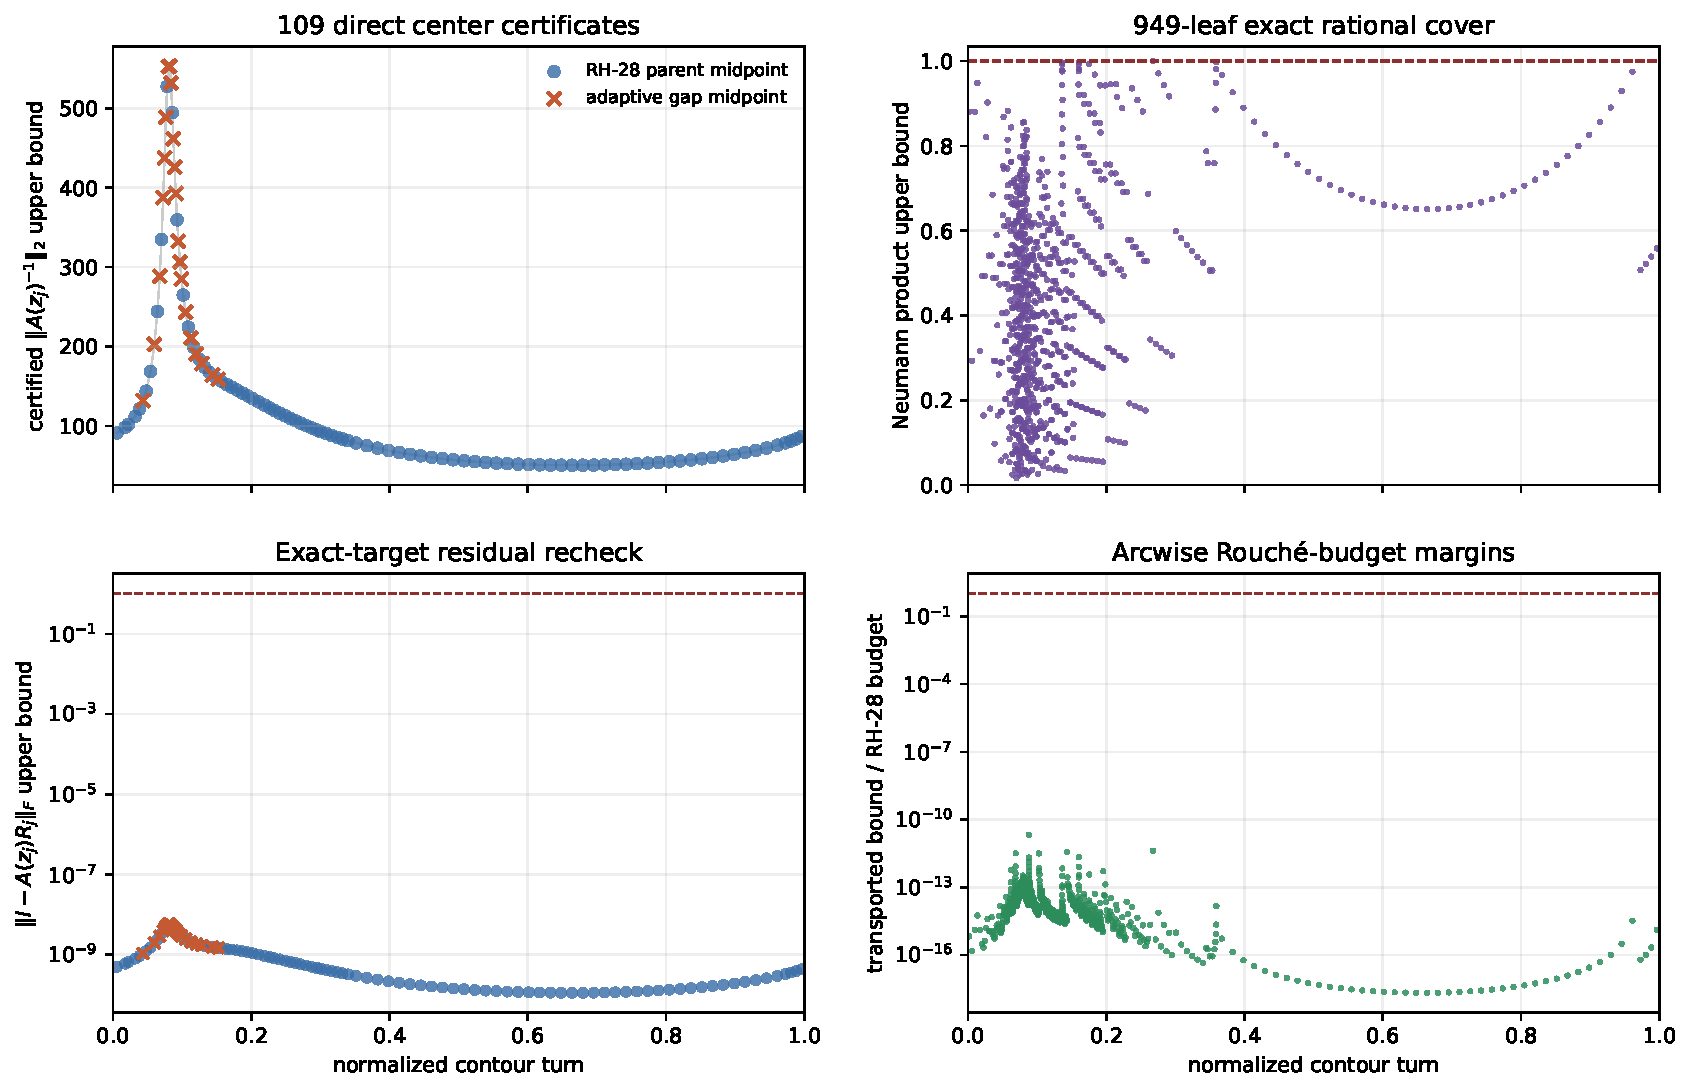
\includegraphics[width=0.99\textwidth]{figures/certified_resolvent_atlas.pdf}
\caption{Top left: the 109 rigorous center inverse bounds, with adaptive
gap-midpoints concentrated near the nonnormal peak.  Bottom left: every
exact-target Frobenius residual remains far below one.  Top right: all 949
leafwise Neumann products are rigorously below one.  Bottom right: the
transported bounds remain many orders of magnitude below the RH-28
conditional budgets.}
\label{fig:atlas}
\end{figure}

\section{Full-boundary Rouch\'e closure and relative winding}
\label{sec:rouche}

For each RH-28 parent, the outward primal--dual theorem gives constants
$\bar\eta_a<1$ and $\bar c_a>0$ with
\begin{equation}
 \norm{F_J(z)^{-1}(F(z)-F_J(z))}_2
 \leq \bar\eta_a+\bar c_a\norm{A(z)^{-1}}_2,\qquad z\in a,
 \label{eq:rh28-bound}
\end{equation}
and the inherited budget is
\begin{equation}
 L_a^-=\operatorname{down}\frac{1-\bar\eta_a}{\bar c_a}.
 \label{eq:rh28-budget}
\end{equation}
Every refined leaf is a subset of its parent, so the parent constants remain
valid on it.

\begin{theorem}[Full stored-boundary Rouch\'e inequality]
\label{thm:full-rouche}
On the complete stored circle,
\begin{equation}
 \norm{F_J(z)^{-1}(F(z)-F_J(z))}_2<1,\qquad z\in\Gamma.
 \label{eq:full-rouche}
\end{equation}
Consequently $F(z)$ is invertible on $\Gamma$ and
\begin{equation}
 \wind_\Gamma\det F=\wind_\Gamma\det F_J=1.
 \label{eq:stored-winding-one}
\end{equation}
\end{theorem}

\begin{proof}
By \cref{thm:full-atlas}, every point lies in a leaf whose transported
inverse upper bound is below the corresponding parent budget.  Substitution
into \cref{eq:rh28-bound,eq:rh28-budget} gives \cref{eq:full-rouche} on each
leaf and hence on $\Gamma$.

For $s\in[0,1]$, define
\[
 F_s(z)=F_J(z)+s(F(z)-F_J(z))
 =F_J(z)\bigl[\Id+sF_J(z)^{-1}(F(z)-F_J(z))\bigr].
\]
The second factor is invertible by the Neumann lemma, uniformly on the
boundary.  Thus $\det F_s$ is a nonvanishing boundary homotopy, so its
winding is constant in $s$.  Apply the independently certified projected
winding \cref{eq:projected-winding-one}; equivalently one may invoke the
boundary form of matrix Rouch\'e theory \citep{GohbergSigal1971}.
\end{proof}

The theorem uses only boundary invertibility and a boundary homotopy.  It
does not assume that $F$ is holomorphic throughout the disk.

\begin{corollary}[Exact relative contour count]
\label{cor:relative-count}
For the exact stored matrices $B$ and $\Maug$,
\begin{equation}
 N_\Gamma(\Maug)-N_\Gamma(B)=1.
 \label{eq:relative-count-one}
\end{equation}
In particular, $\Maug$ has at least one eigenvalue in the circle, counted
algebraically.
\end{corollary}

\begin{proof}
The atlas excludes $\spec B$ from the boundary.  The full Rouch\'e
inequality and \cref{eq:projected-winding-one} exclude zeros of $\det F$
from the boundary.  Hence \cref{prop:stored-schur} applies, and
\cref{eq:stored-winding-one} gives \cref{eq:relative-count-one}.  Since
$N_\Gamma(B)$ is a nonnegative integer,
$N_\Gamma(\Maug)=N_\Gamma(B)+1\geq1$.
\end{proof}

\begin{remark}[Why this is not yet a one-zero theorem]
\label{rem:not-one-zero}
The rational function $F$ may have poles at interior complement
eigenvalues.  If $q=N_\Gamma(B)$, the present theorem gives
$N_\Gamma(\Maug)=q+1$ and boundary winding one.  It gives exactly one
augmented eigenvalue, or exactly one ordinary zero of $\det F$, only after
proving $q=0$.
\end{remark}

\section{Provenance, reproducibility, and evidence level}
\label{sec:reproducibility}

The committed archive contains one JSON record for every center.  Each
record stores the center, sparse dimensions, LU fill, $\rho_j$,
$\varepsilon_j$, $M_j$, timings, and SHA-256 hashes of the streamed trial
inverse, residual centers, and residual radii.  The aggregate center table
and manifest contain 109 rows and verify that every center certificate is
admissible.

The leaf ledger contains all 949 final rational intervals, the winning
center identifier, the Arb distance upper bound, Neumann product upper
bound, transported inverse upper bound, inherited budget lower bound, and
their ratio.  Independent archive tests reconstruct the exact rational
partition from integer endpoints and require every row to be closed.

The dependency manifest hashes the consumed RH-28 arc and scale archives,
the RH-32 projected count, the RH-27 componentwise arithmetic and factor
graph, the RH-28 rational geometry, and the RH-30 Frobenius--Neumann helper.
These hashes establish object provenance; they do not replace the
mathematical assumptions of the source theorems.

The rigorous computation concerns exact dyadic inputs.  It assumes the
standard IEEE round-to-nearest model used by the outward arithmetic, with no
overflow or harmful underflow.  Sparse LU is outside the trusted base: any
LU error merely changes the trial matrix and is remeasured by the
exact-target residual.

\section{Scope, limitations, and next gate}
\label{sec:limitations}

The paper proves four concrete statements at $\sigma=10^{-2}$:

\begin{enumerate}
 \item 109 exact-target center inverse bounds for the stored complement
       family;
 \item a complete rational boundary resolvent atlas;
 \item the full RH-28 matrix Rouch\'e inequality on the stored circle; and
 \item stored Feshbach winding one and augmented-block-minus-complement
       count one.
\end{enumerate}

The following statements are not proved.

\begin{enumerate}
 \item The interior complement count $N_\Gamma(B)$ is not known.  Therefore
       no ordinary one-zero count for $F$ and no exactly-one count for
       $\Maug$ follows.
 \item Because exact idempotence of the serialized $Q$ is not assumed, the
       augmented stored block is not silently identified with the original
       physical two-step discretization.  Such an identification would need
       an exact packet-pair correction or a separate perturbation theorem.
 \item The same full atlas has not been computed at
       $\sigma=4\times10^{-3}$ or smaller scales.  The all-column certificate
       has quadratic-like cost, although the sparse factorization itself
       remains favorable at the next stored scale.
 \item The stored finite factors are not enclosed relative to an exact
       Gaussian integral operator, exact critical constants, or a zero-noise
       limit.
 \item No self-adjoint Hilbert--P\'olya operator, prime-power trace formula,
       zeta-zero identification, or statement about the Riemann hypothesis
       is obtained.
\end{enumerate}

The immediate spectral gate is now narrower than in RH-32.  Boundary
resolvent control is no longer missing at the coarsest stored scale.  What
remains is an interior complement count.  Natural routes include a contour
argument principle for the complement determinant, a pole-free homotopy, a
validated sparse inertia count for an interior family, or a Schur
self-energy exclusion.  Each route addresses a different question from
adding more boundary centers \citep{SjoestrandZworski2007,TrefethenEmbree2005}.

\section{Conclusion}
\label{sec:conclusion}

A single local inverse bound could not traverse the RH-28 contour.  A finite
atlas can.  The practical reason is that sparse LU need not be validated as
a factorization: it only proposes local right inverses, while the exact
stored-factor graph certifies every residual independently.  Exact rational
gap geometry then places new centers only where previous charts fail.

At $\sigma=10^{-2}$, 109 charts cover the full boundary.  This closes the
conditional resolvent gate left by RH-28 and RH-32, promotes projected
winding one to exact stored Feshbach winding one, and yields an exact
relative count for the augmented stored block.  The result does not jump the
last wall.  Interior complement poles still decide whether relative count
one becomes an ordinary one-zero theorem.  That distinction is the next
problem, not a caveat to be hidden by numerical evidence.

\appendix

\section{Explicit low-rank channels}
\label{app:channels}

Write a channel column as
$x=(x_{\rm top},x_{\rm bottom})^{\mathsf T}$ and a channel row as
$y=(y_{\rm left},y_{\rm right})$.  The $2p+2m$ channels in
\cref{eq:channel-rank} are
\begin{align*}
 x_{{\rm tp},k}&=(t(C_{\rm p})_k,0)^{\mathsf T},
 &y_{{\rm tp},k}&=(0,(L_{\rm p}^{\mathsf T})_k),\\
 x_{{\rm tk},k}&=(tV_k,0)^{\mathsf T},
 &y_{{\rm tk},k}&=(0,(WU)_k),\\
 x_{{\rm bp},k}&=(0,t^{-1}(C_{\rm p})_k)^{\mathsf T},
 &y_{{\rm bp},k}&=((L_{\rm p}^{\mathsf T})_k,0),\\
 x_{{\rm bk},k}&=(0,t^{-1}(UV)_k)^{\mathsf T},
 &y_{{\rm bk},k}&=(W_k,0).
\end{align*}
The first and third families have $p$ channels; the second and fourth have
$m$ channels.  Summing $xy$ gives precisely the corrections in
\cref{eq:top-correction,eq:bottom-correction}.

\section{Reproduction}
\label{app:reproduction}

From this paper directory, run the fast tests and rebuild the compact
archive by
\begin{verbatim}
PYTHONDONTWRITEBYTECODE=1 python -m pytest -q -p no:cacheprovider
PYTHONDONTWRITEBYTECODE=1 python experiments/build_archive.py
MPLBACKEND=Agg python experiments/make_figures.py
\end{verbatim}
The expensive center certificates are resumable.  One parent-center batch
is run with
\begin{verbatim}
OPENBLAS_NUM_THREADS=1 OMP_NUM_THREADS=1 \
python experiments/run_atlas_batch.py --sigma 0.01 \
  --workers 8 --chunk-size 256 --arcs <arc identifiers>
\end{verbatim}
After a partial atlas, generate rational gap midpoints and certify them by
\begin{verbatim}
python experiments/audit_refined_atlas.py \
  --sigma 0.01 --max-extra-refinement 8
OPENBLAS_NUM_THREADS=1 OMP_NUM_THREADS=1 \
python experiments/run_atlas_batch.py --sigma 0.01 \
  --workers 8 --chunk-size 256 \
  --target-file results/refined_atlas_sigma_1e-02.json
\end{verbatim}
The final audit is rerun until its status is
\texttt{full\_refined\_atlas}.  The manuscript is built with
\begin{verbatim}
latexmk -pdf -interaction=nonstopmode -halt-on-error main.tex
\end{verbatim}

\bibliographystyle{plainnat}
\bibliography{references}

\end{document}
